\documentclass[11pt, a4paper]{article}

\usepackage[top = 1 in, bottom = 1 in, left = 1 in, right = 1 in]{geometry}

\usepackage{amsmath, amssymb, amsfonts}
\usepackage{enumerate}
\usepackage{multirow}
\usepackage{hhline}
\usepackage{array}
\usepackage{longtable}
\usepackage{graphicx}
\usepackage{tabularray}
\usepackage{undertilde}
\usepackage{dingbat}
\usepackage{fontawesome5}
\usepackage[colorlinks=true, linkcolor=blue, urlcolor=red]{hyperref}
\usepackage{tasks}
\usepackage{bbding}
\usepackage{twemojis}
% how to use bull's eye ----- \scalebox{2.0}{\twemoji{bullseye}}
\usepackage{customdice}
% how to put dice face ------ \dice{2}

\title{MSMS 201 : CLUSTERING}
\author{Ananda Biswas}
\date{\today}


\begin{document}

\maketitle

$\bullet$ \textbf{Clustering :} Partition data $\chi$ into $k$-groups such that observations in each group are similar and observations in between different groups are far away.

\begin{figure}[!htbp]
\centering
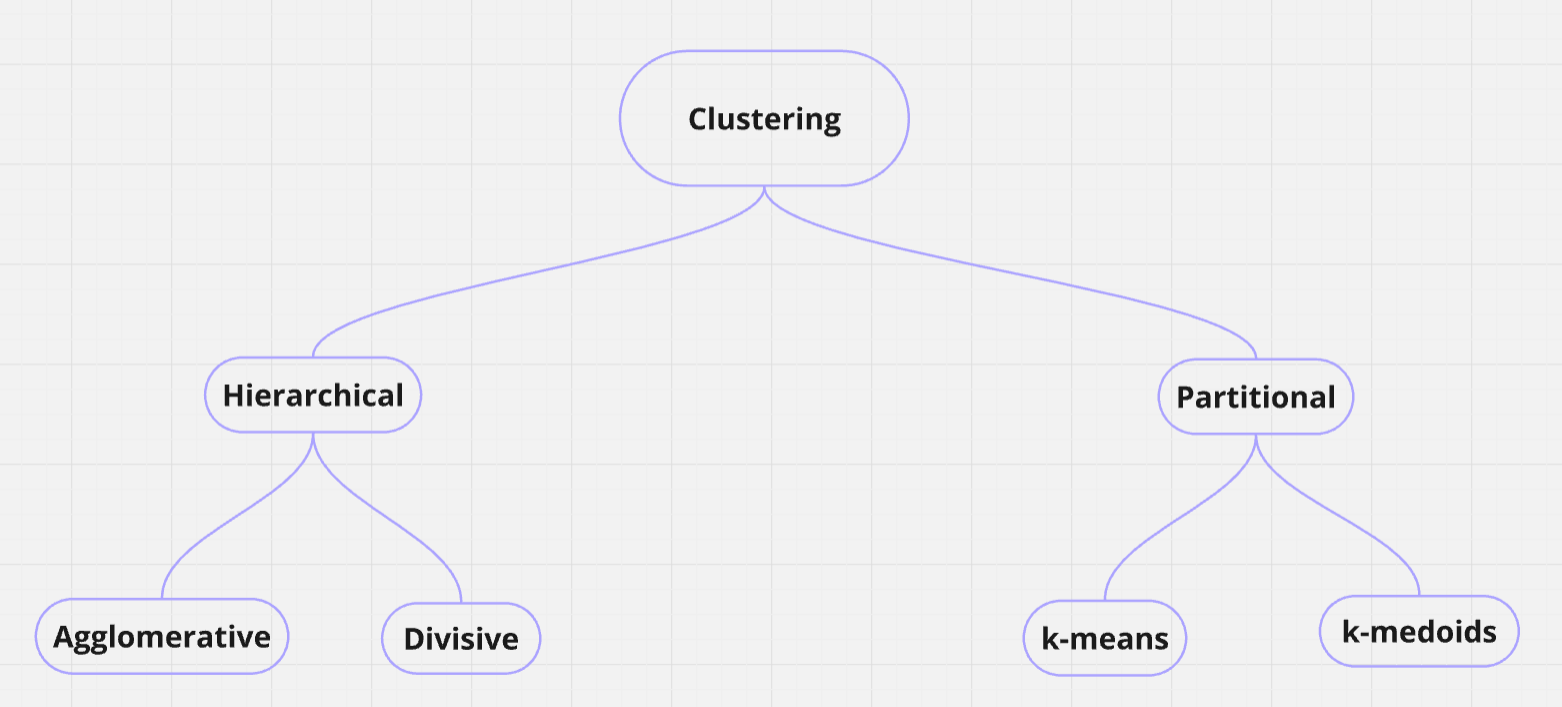
\includegraphics[scale=0.4]{image1.png}
\end{figure}

$\bullet$ \textbf{Partitional Clustering :} It is simply a division of data objects into non-overlapping subsets such that each object is in only one set. \\

Two well-known partitional clustering techniques are -

\begin{enumerate}[(i)]
\item $k$-means
\item $k$-medoids
\end{enumerate}

In partitional clustering algorithm, our objective is to partition $\chi$ in $k$-clusters such that cost function is minimum. \\

\leftpointright \hspace{0.2cm} \textbf{\textcolor{blue}{$k$-means clustering :-}} defines a prototype in terms of centroid which is usually the mean of a group of points. It is applied when the objects are in continuous $n$-dimensional space. Centroid may not be an actual data-point. \\

\faArrowAltCircleRight[regular] \hspace{0.2cm} \textbf{Algorithm for $k$-means clustering :-} \\

The $k-$means clustering algorithm is as follows :

\begin{enumerate}[(1)]
\item select $k$ points as initial centroids
\item calculate the distance of each data-point from each of the centroids
\item assign each of the data-points to its closest centroid
\item relocate the centroids to the average location of the data-points of similar group
\end{enumerate}

And we repeat this procedure until the assignments don't change after the centroid locations were recomputed. \\

For some type of combinations of proximity measure and types of centroids, $k$-mean always converges to a solution. \\

\scalebox{2.0}{\twemoji{bullseye}} \hspace{0.5cm} \href{https://github.com/sakunisgithub/R-programming/blob/master/msc_sem_2_practicals/rakesh_sir_practicals/practical_01/practical_01.pdf}{\underline{an example : $k$-means clustering on a 1D data}} \\

\scalebox{2.0}{\twemoji{bullseye}} \hspace{0.5cm} \href{https://github.com/sakunisgithub/R-programming/blob/master/msc_sem_2_practicals/rakesh_sir_practicals/practical_02/practical_02.pdf}{\underline{an example : $k$-means clustering on $iris$ dataset}} \\

\leftpointright \hspace{0.2cm} \textbf{\textcolor{blue}{$k$-medoids clustering :-}} It defines a prototype in terms of medoids which are the most representative points of a group of points and can be applied to a wide range of data. It requires only a proximity measure for a pair of objects. Medoid must be an actual data-point while centroids mostly never correspond to any actual data-point. \\

\faArrowAltCircleRight[regular] \hspace{0.2cm} \textbf{Algorithm for $k$-medoids clustering :-} \\

The $k-$medoids clustering algorithm is as follows :

\begin{enumerate}[(1)]
\item randomly select $k$ data-points as initial medoids belonging to $k$ clusters
\item calculate the distance of each data-point from each of the medoids using \underline{Manhattan Distance} $M$ given by

$$M((X_1, Y_1), (X_2, Y_2)) = |X_1 - X_2|+|Y_1 - Y_2|$$

\item assign each of the data-points to the cluster from whose medoid the distance $M$ is minimum
\item calculate the total cost $S$ given by

$$S = \sum\limits_{i = 1}^{k} \sum\limits_{j} M(C_i, X_{ij})$$

where $C_i$ is the medoid of $i$-th cluster and $X_{ij}$ is the $j$th data-point in $i$th cluster.

\end{enumerate}

And we repeat this procedure and obtain a new total cost. \\

Let $G = \text{new total cost} - \text{old total cost}$. We stop if $G > 0$. \\


$\bullet$ \textbf{\textcolor{orange}{choosing the initial centroid :}} When random initialization of centroid is used, different runs of $k$-means typically produce different total $SSE$. One effective approach is to take a sample of points and cluster them using a hierarchical clustering. $k$ clusters are to be extracted from hierarchical clustering technique and centroid of these clusters can be used as initial values.

$$SSE = \sum\limits_{i = 1}^{k} \sum\limits_{x \in c_i} (x - m_i)^2$$

$$\dfrac{\partial}{\partial m_k} (SSE) = -2 \cdot \sum\limits_{x \in c_k}(x - m_k)$$

and equating the partial derivative to $0$ will yield $m_k = \dfrac{1}{n_k}\sum\limits_{x \in m_k} x_k$; where $m_i$ is the centroid of cluster $c_i$ consisting of $n_i$ data-points. Also if we calculate second derivative, it is greater than 0 at obtained $m_k$. Hence, mean is the best centroid for minimizing $SSE$ of clusters. \\

If we use Sum of Absolute Errors $SAE = \sum\limits_{i = 1}^{k} \sum\limits_{x \in c_i} |x - m_i|$ as our cost function, then $m_k = \text{median}\{x : x \in c_k \}$ minimizes $SAE$. \\

\leftpointright \hspace{0.2cm} \textbf{\textcolor{blue}{Hierarchical clustering :-}} In Hierarchical clustering the observation vectors are grouped on the basis of their mutual distances. It is usually visualized through \textit{dendograms}. There are two basic approaches for generating hierarchical clusters - 

\begin{enumerate} [(a)]
\item Agglomerative Hierarchical Clustering
\item Divisive Hierarchical Clustering
\end{enumerate}

$\bullet$ \textbf{Distance Matrix} in a bivariate dataset :

\begin{table}[!htbp]
\def\arraystretch{1.5}

\begin{center}
\begin{tabular}{|c|c|c|}

\hline

point & $x$ & $y$ \\

\hline

$A$ & 1 & 2 \\

$B$ & 3 & 1 \\

$C$ & 2 & 2 \\

$D$ & 1 & 3 \\

\hline

\end{tabular}
\end{center}

\end{table}

The distance matrix is given as 

\begin{gather*}
\begin{pmatrix}
0 & \sqrt{5} & 1 & 1 \\
\sqrt{5} & 0 & \sqrt{3} & 2\sqrt{2} \\
1 & \sqrt{3} & 0 & \sqrt{2} \\
1 & 2\sqrt{2} & \sqrt{2} & 0 \\
\end{pmatrix}
\end{gather*}

Notice that, a distance matrix will always be symmetric.
\end{document}